\hypertarget{slider_8hpp}{
\section{/home/arnaud/programmation/sfml/sfgui/slider.hpp File Reference}
\label{slider_8hpp}\index{/home/arnaud/programmation/sfml/sfgui/slider.hpp@{/home/arnaud/programmation/sfml/sfgui/slider.hpp}}
}
{\tt \#include \char`\"{}object.hpp\char`\"{}}\par


Include dependency graph for slider.hpp:\nopagebreak
\begin{figure}[H]
\begin{center}
\leavevmode
\includegraphics[width=339pt]{slider_8hpp__incl}
\end{center}
\end{figure}


This graph shows which files directly or indirectly include this file:\nopagebreak
\begin{figure}[H]
\begin{center}
\leavevmode
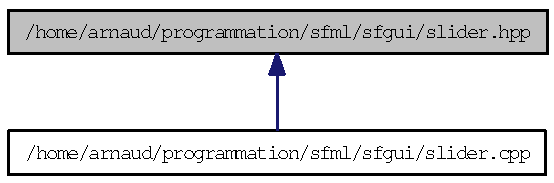
\includegraphics[width=151pt]{slider_8hpp__dep__incl}
\end{center}
\end{figure}
\subsection*{Classes}
\begin{CompactItemize}
\item 
class \hyperlink{classSlider}{Slider}
\end{CompactItemize}


\subsection{Detailed Description}
\begin{Desc}
\item[Author:]TANGUY Arnaud $<$\href{mailto:arn.tanguy@gmail.com}{\tt arn.tanguy@gmail.com}$>$ \end{Desc}
\begin{Desc}
\item[Version:]0.1 \end{Desc}
\begin{Desc}
\item[Date:]Created: sam 10 jan 2009 19:45:30 CET \par
 Last Update: sam 10 jan 2009 19:45:30 CET\end{Desc}
Copyright (C) 2008 TANGUY Arnaud

This program is free software; you can redistribute it and/or modify it under the terms of the GNU General Public License as published by the Free Software Foundation; either version 2 of the License, or (at your option) any later version.

This program is distributed in the hope that it will be useful, but WITHOUT ANY WARRANTY; without even the implied warranty of MERCHANTABILITY or FITNESS FOR A PARTICULAR PURPOSE. See the GNU General Public License for more details.

You should have received a copy of the GNU General Public License along with this program; if not, write to the Free Software Foundation, Inc., 51 Franklin Street, Fifth Floor, Boston, MA 02110-1301 USA. 